



%Autor: Nico Schrodt
%Oktober 2021 - Mai 2022


\documentclass[12pt]{article}

\usepackage{multicol}
\usepackage{geometry}
\usepackage{blindtext}
\usepackage{setspace}
\usepackage{hyperref}
\usepackage[headsepline=0.8pt, footsepline =0.8pt]{scrlayer-scrpage}
\usepackage{listings}
\usepackage{subcaption}
\usepackage{tabularx}
\usepackage{xurl} %Formats \url{}-entrys better
\usepackage{color, colortbl}
%\usepackage{pdfpages}
\usepackage{amssymb}

\geometry{a4paper, top=25mm, left=35mm, right=25mm, bottom=25mm, headsep=13mm, footskip=12mm, head=14.5pt}

%encoding
%--------------------------------------
\usepackage[utf8]{inputenc}
\usepackage[T1]{fontenc}
%--------------------------------------

%German-specific commands
%--------------------------------------
\usepackage[ngerman]{babel}
%--------------------------------------

%Hyphenation rules
%--------------------------------------
\usepackage{hyphenat}
%--------------------------------------

\usepackage{graphicx}
\graphicspath{ bilder/}

\newcommand{\Autor}{Nico Schrodt}

\newcommand{\Bearbeitungszeitraum}{5 + 6 Semester}
\newcommand{\Kurs}{TINF19B3}
\newcommand{\Betreuer}{Daniel Lindner}

\newcommand{\DHBWLogoDeckblatt}{
\includegraphics[width=4.5cm]{Logos/dhbw-logo}}

\newcommand{\Titel}{Entwerfen und Implementieren einer Verschlüsselungssoftware}
\newcommand{\ArtArbeit}{Ausarbeitung}
\newcommand{\Abschluss}{Bachelor of Science}
\newcommand{\Studiengang}{Studiengang Informationstechnik}

\newcommand{\Ort}{Karlsruhe}

%\newcommand{\Abgabedatum}{16.02.2021}


\begin{document}
\onehalfspacing
\pagenumbering{Roman}
	\begin{titlepage}
		{\DHBWLogoDeckblatt}\\[2cm]
		\begin{center}
			\vspace*{-2cm}
			{\Huge \Titel}\\[2cm]
			{\Huge \ArtArbeit}\\[2cm]
			{\Large \Abschluss}\\[0.5cm]
			{\large \Studiengang}\\[0.5cm]
			{\large an der}\\[0.5cm]
			{\large Dualen Hochschule Baden-Württemberg Karlsruhe}\\[0.5cm]
			{\large von}\\[0.5cm]
			{\large\bfseries \Autor}\\[1cm]
			{\large Abgabedatum \today}
			\vfill
		\end{center}
		\begin{tabular}{l@{\hspace{1cm}}l}
			Bearbeitungszeitraum & \Bearbeitungszeitraum \\
			Kurs & \Kurs \\
%			Ausbildungsfirma & \Ausbildungsfirma \\
			Dozent & \Betreuer \\
		\end{tabular}
	\end{titlepage}

\newpage

\thispagestyle{empty}
\tableofcontents

\newpage

%\thispagestyle{empty}
\thispagestyle{plain}
\cleardoublepage
\addcontentsline{toc}{section}{\listfigurename}
\listoffigures

\addcontentsline{toc}{section}{\listtablename}
\listoftables

\addcontentsline{toc}{section}{Listings}
\lstlistoflistings

\newpage

%\thispagestyle{empty}
\thispagestyle{plain}
\cleardoublepage
\section*{Abkürzungsverzeichnis}
\addcontentsline{toc}{section}{Abkürzungsverzeichnis}

\newpage
\pagenumbering{arabic}

%% Kopf und Fusszeilen==================================================== 
\pagestyle{scrheadings} % Seite mit Headern 

% loescht voreingestellte Stile 
\clearpairofpagestyles
%\clearscrheadings 
\clearmainofpairofpagestyles
%\clearscrplain 

% %%% Kopfzeile 
% einseitig: Bei einseitigem Layout, nur folgende Zeilen verwenden !!! 
%\ohead[] {
\includegraphics[height=0.5cm]{Logos/Firmenlogokopfzeile}}
\ihead[]{\leftmark} % links: Kapitel
%\chead[]{} % mitte: 

% %%% Fusszeile 
%\cfoot[]{} % mitte: 
\cfoot[\pagemark]{\pagemark} % rechts: Seitenzahl


% Angezeigte Abschnitte im Header 
\automark{section}  % Inhalt von [\rightmark]{\leftmark} 

\section{Einführung}
Dieses Kapitel befasst sich vorwiegend mit relevanten Grundlagen der Arbeit. Unter anderem wird das Ziel spezifiziert, elementare Aspekte der Arbeitsweise eines Prozessors werden erläutert und die verschiedenen Werkzeuge mit denen das Ziel realisiert wird werden aufgeführt.

\subsection{Ziel der Arbeit}
In dieser Arbeit soll ein Simulationsprogramm geschrieben werden, mit dem mehrere unterschiedliche 8-Bit Prozessoren simuliert werden können. Dazu sollen die Grundlegenden Eigenschaften in kurzen Lernprogrammen erläutert werden. Ebenfalls soll es eine interaktive Einweisung geben wie der Simulator verwendet werden kann.

\subsection{Repository}
Der Quellcode kann in folgendem GitHub-Repository abgerufen werden:\\ \url{https://github.com/NicoSchrodt/EncryptionService}

\newpage

\section{Clean Architecture}
Der Sinn einer Clean Architecture ist es das Programm in klar definierte Schichten zu zerlegen die unabhängig voneinander ausgetauscht werden können. Dadurch soll idealerweise die Langlebigkeit und Wartbarkeit eines Projekts gewährleistet werden können.

\subsection{Geplante Schichtenarchitektur}
Für dieses Projekt sind zwei Schichten vorgesehen. Einmal die Benutzeroberfläche (GUI) welche mit Qt implementiert wird und die Logik, welche unter anderem die Verschlüsselung vornimmt. Der Benutzer soll ausschließlich mit der von Qt generierten Oberfläche interagieren z.B. durch Textfelder oder Knöpfe, welche vorkonfigurierte Befehle ausführen.

\subsection{Umsetzung}
Platzhalter

\subsubsection{Benutzeroberfläche}
Platzhalter

\subsubsection{Verschlüsselungsdienst}
Platzhalter

\newpage

\section{Entwurfsmuster}
Das für den Umfang dieses Programmentwurfs verwendete Entwurfsmuster ist der Dekorierer. Aufgabe des Dekorierers ist es eine Klasse oder Funktion um einen oder mehrere Aspekte zu erweitern ohne die Klasse selbst zu verändern. Das Entwurfsmuster wurde in der Klasse 'EncrypterInterface.py' angewendet.
\begin{center}
	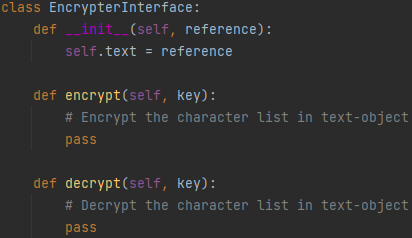
\includegraphics[width=10cm]{bilder/Decorator_before.png}
\end{center}
'EncrypterInterface' dient wie der Name bereits verrät als Interface für konkrete Encrypter. Dabei ist aber nicht gewährleistet, dass die konkrete Implementierung die im Interface beschriebenen Funktion selbst implementiert. Der Dekorierer soll hier die Aufgabe Übernehmen, auf eine konkrete Implementierung zu kontrollieren und bei Fehlen dieser eine Exception auszulösen.
\begin{center}
	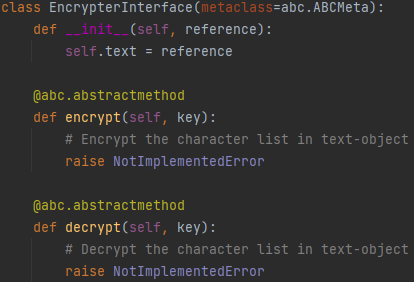
\includegraphics[width=10cm]{bilder/Decorator_after.png}
\end{center}
Die Funktion des Dekorierers beschränkt sich hier auf konkrete Implementierungen des EncrypterInterfaces, Also Klassen die von 'EncrypterInterface' erben. Das Interface selbst könnte potentiell immer noch instantiiert und verwendet werden ohne die Exception auszulösen.

\newpage

\section{Programming Principles}
In diesem Abschnitt werden kurz einige Programming Principles erläutert und deren Anwendung an Beispielen in diesem Projekt aufgezeigt.

\subsection{SOLID}
\subsubsection{Single Responsible Principle}
Platzhalter

\subsubsection{Open/Closed Principle}
Platzhalter

\subsubsection{Liskov Substitution Principle}
Platzhalter

\subsubsection{Interface Segregation Principle}
Platzhalter

\subsubsection{Dependency Inversion Principle}
Platzhalter

\subsection{GRASP}

\subsubsection{Low Coupling}
Platzhalter

\subsubsection{High Cohesion}
Platzhalter

\subsection{DRY}
DRY steht für 'Don't repeat yourself'. Zentraler Angelpunkt dieses Prinzips ist das Vermeiden von Code Duplikaten, sowie das Strukturieren des Programmcodes in einer Weise das nur logisch verknüpfte Elemente sich gegenseitig beeinflussen. Oder in anderen Worten, jedes logische Konstrukt im Quellcode muss durch eine klare von anderen Aspekten getrennte Struktur repräsentiert werden. Dadurch lassen sich z.B. einige Code Smells verhindern wie "Duplicated Code" oder "Shotgun Surgery".\\
Das Prinzip wurde angewendet hinsichtlich dem vermeiden von Code Duplikaten, welche sich unter anderem in zahlreichen Klassen die für die Verschlüsselung zuständig sind befanden, da der Prozess der Ver- und Entschlüsselung je nach Verfahren recht ähnlich ist (bspw. Vigenère- oder Caesar-Chiffre).

\newpage

\section{Refactoring}
Das Ziel von Refactoring ist das Verbessern der Codequalität. Für diese Arbeit ist es unterteilt in das Identifizieren von 3 verschiedenen Code Smells und das Anwenden von 2 Refactorings.

\subsection{Code Smells}
Unter 'Code Smells' versteht man Stellen im Programmcode, welche Verbesserungspotential aufweisen bspw. bezüglich der Übersichtlichkeit.\\ (\textbf{Anmerkung: }Die hier aufgelisteten Code Smells sind womöglich nicht mehr in der neuesten Version des Projekts zu finden, sondern nur noch in älteren Commits)

\subsubsection{Code Smells 1 Duplicated Code}
Dieses Beispiel für einen 'Duplicated Code'- Code Smells ist in der 'Caesar-Encrypter.py'- Datei zu finden. Ausschlaggebend ist hierbei, dass das Verfahren zum Ver- und Entschlüsseln effektiv gleich ist mit der Ausnahme, welcher der Starttext ist und in welche Richtung (Positiv/Negativ) der Schlüssel anzuwenden ist.
\begin{center}
	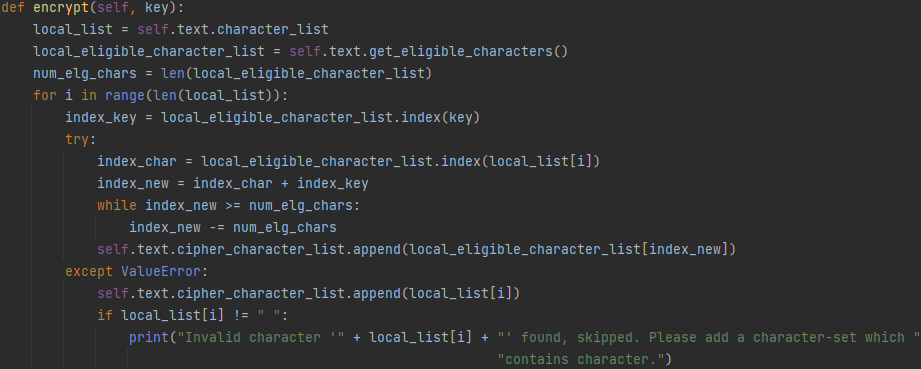
\includegraphics[width=15cm]{bilder/CodeSmells1_a.png}
\end{center}
\begin{center}
	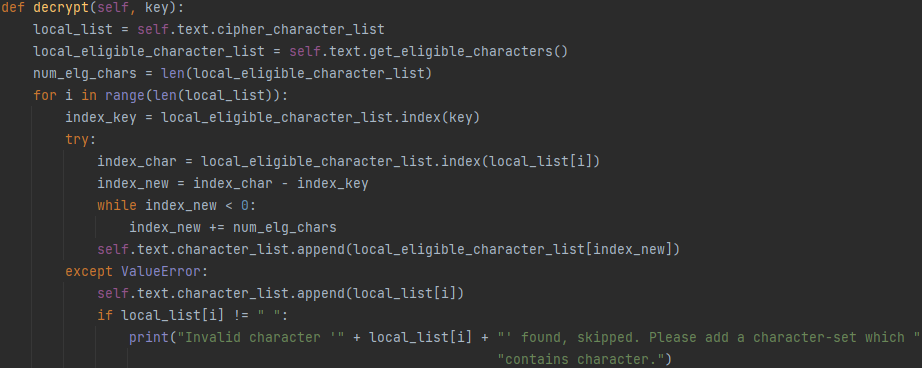
\includegraphics[width=15cm]{bilder/CodeSmells1_b.png}
\end{center}

\subsubsection{Code Smells 2 Long Method}
Platzhalter

\subsubsection{Code Smells 3 Large Class}
Der dritte Code Smells zeigt eine 'Large Class'. Dieser bezeichnet eine große Klasse die unter anderem zu viele Instanzvariablen, Methoden oder allgemein Codezeilen aufweist.

\subsection{Angewendete Refactorings}
Platzhalter

\subsubsection{Refactoring 1}
Platzhalter

\subsubsection{Refactoring 2}
Platzhalter

\newpage

\section{Unit Tests}
Platzhalter

\subsection{Verwendete Unit Tests und getesteter Code}
Platzhalter

\subsubsection{Mocks}
Platzhalter

\subsubsection{Code Coverage}
Platzhalter

\subsection{Anwendung der ATRIP-Regeln}
Platzhalter


%\newpage
%\thispagestyle{empty}
%
%\section*{Anhang}
%\addcontentsline{toc}{section}{Anhang}


\end{document}